% Buffon's needle: left, 40 needles of length 0.8 on lines 1 apart (crossing needles in orange); right, the favourable region x <= (l/2) sin(theta) in the rectangle of (theta, x). Generated by a short script.
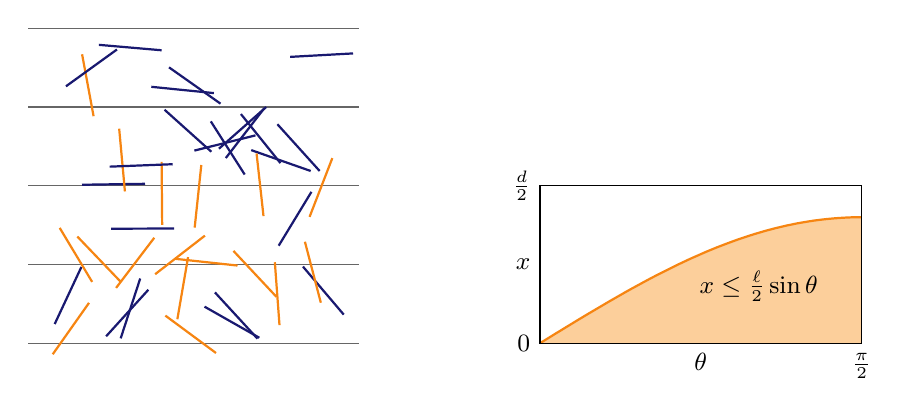
\begin{tikzpicture}
\draw[black!60] (0,0.00)--(4.2,0.00);
\draw[black!60] (0,1.00)--(4.2,1.00);
\draw[black!60] (0,2.00)--(4.2,2.00);
\draw[black!60] (0,3.00)--(4.2,3.00);
\draw[black!60] (0,4.00)--(4.2,4.00);
\draw[BurntOrange,thick] (1.116,0.702)--(1.601,1.339);
\draw[BurntOrange,thick] (1.894,0.304)--(2.030,1.093);
\draw[MidnightBlue,thick] (1.694,3.720)--(0.897,3.789);
\draw[BurntOrange,thick] (2.658,0.986)--(1.862,1.072);
\draw[MidnightBlue,thick] (1.052,1.454)--(1.852,1.456);
\draw[BurntOrange,thick] (1.701,1.504)--(1.694,2.304);
\draw[MidnightBlue,thick] (0.683,2.012)--(1.483,2.024);
\draw[MidnightBlue,thick] (1.174,0.061)--(1.422,0.821);
\draw[BurntOrange,thick] (0.311,-0.141)--(0.772,0.512);
\draw[BurntOrange,thick] (1.228,1.927)--(1.155,2.724);
\draw[MidnightBlue,thick] (3.203,2.287)--(2.701,2.910);
\draw[MidnightBlue,thick] (3.181,1.238)--(3.597,1.922);
\draw[MidnightBlue,thick] (4.007,0.363)--(3.489,0.973);
\draw[MidnightBlue,thick] (2.935,0.069)--(2.239,0.464);
\draw[MidnightBlue,thick] (3.701,2.187)--(3.164,2.781);
\draw[BurntOrange,thick] (3.191,0.230)--(3.132,1.028);
\draw[MidnightBlue,thick] (2.442,3.042)--(1.788,3.503);
\draw[MidnightBlue,thick] (3.587,2.187)--(2.832,2.452);
\draw[MidnightBlue,thick] (2.422,2.470)--(3.022,2.999);
\draw[MidnightBlue,thick] (0.336,0.243)--(0.675,0.968);
\draw[BurntOrange,thick] (0.830,2.883)--(0.684,3.669);
\draw[MidnightBlue,thick] (2.749,2.142)--(2.319,2.817);
\draw[BurntOrange,thick] (2.385,-0.125)--(1.742,0.350);
\draw[BurntOrange,thick] (2.988,1.614)--(2.900,2.409);
\draw[MidnightBlue,thick] (2.912,0.057)--(2.371,0.645);
\draw[MidnightBlue,thick] (0.989,0.087)--(1.526,0.679);
\draw[BurntOrange,thick] (3.153,0.588)--(2.606,1.172);
\draw[BurntOrange,thick] (3.573,1.604)--(3.862,2.350);
\draw[MidnightBlue,thick] (2.326,2.431)--(1.731,2.965);
\draw[MidnightBlue,thick] (2.110,2.446)--(2.886,2.639);
\draw[BurntOrange,thick] (1.178,0.776)--(0.624,1.354);
\draw[MidnightBlue,thick] (1.035,2.242)--(1.835,2.273);
\draw[BurntOrange,thick] (0.812,0.778)--(0.400,1.464);
\draw[MidnightBlue,thick] (2.509,2.351)--(2.998,2.984);
\draw[BurntOrange,thick] (2.114,1.468)--(2.198,2.263);
\draw[MidnightBlue,thick] (0.479,3.262)--(1.127,3.730);
\draw[MidnightBlue,thick] (3.326,3.636)--(4.125,3.680);
\draw[MidnightBlue,thick] (2.358,3.176)--(1.563,3.256);
\draw[BurntOrange,thick] (1.612,0.876)--(2.244,1.366);
\draw[BurntOrange,thick] (3.716,0.514)--(3.514,1.288);
\fill[BurntOrange!35] (6.5,0) -- plot coordinates {(6.500,0.000) (6.568,0.042) (6.636,0.084) (6.704,0.126) (6.772,0.167) (6.840,0.209) (6.908,0.250) (6.976,0.292) (7.045,0.333) (7.113,0.374) (7.181,0.414) (7.249,0.454) (7.317,0.494) (7.385,0.534) (7.453,0.573) (7.521,0.612) (7.589,0.651) (7.657,0.689) (7.725,0.726) (7.793,0.763) (7.861,0.800) (7.929,0.836) (7.997,0.871) (8.066,0.906) (8.134,0.940) (8.202,0.974) (8.270,1.007) (8.338,1.039) (8.406,1.071) (8.474,1.101) (8.542,1.131) (8.610,1.161) (8.678,1.189) (8.746,1.217) (8.814,1.243) (8.882,1.269) (8.950,1.294) (9.019,1.319) (9.087,1.342) (9.155,1.364) (9.223,1.386) (9.291,1.406) (9.359,1.426) (9.427,1.444) (9.495,1.462) (9.563,1.478) (9.631,1.494) (9.699,1.508) (9.767,1.522) (9.835,1.534) (9.903,1.545) (9.971,1.556) (10.040,1.565) (10.108,1.573) (10.176,1.580) (10.244,1.586) (10.312,1.591) (10.380,1.595) (10.448,1.598) (10.516,1.599) (10.584,1.600)} -- (10.584,0) -- cycle;
\draw[BurntOrange,thick] plot coordinates {(6.500,0.000) (6.568,0.042) (6.636,0.084) (6.704,0.126) (6.772,0.167) (6.840,0.209) (6.908,0.250) (6.976,0.292) (7.045,0.333) (7.113,0.374) (7.181,0.414) (7.249,0.454) (7.317,0.494) (7.385,0.534) (7.453,0.573) (7.521,0.612) (7.589,0.651) (7.657,0.689) (7.725,0.726) (7.793,0.763) (7.861,0.800) (7.929,0.836) (7.997,0.871) (8.066,0.906) (8.134,0.940) (8.202,0.974) (8.270,1.007) (8.338,1.039) (8.406,1.071) (8.474,1.101) (8.542,1.131) (8.610,1.161) (8.678,1.189) (8.746,1.217) (8.814,1.243) (8.882,1.269) (8.950,1.294) (9.019,1.319) (9.087,1.342) (9.155,1.364) (9.223,1.386) (9.291,1.406) (9.359,1.426) (9.427,1.444) (9.495,1.462) (9.563,1.478) (9.631,1.494) (9.699,1.508) (9.767,1.522) (9.835,1.534) (9.903,1.545) (9.971,1.556) (10.040,1.565) (10.108,1.573) (10.176,1.580) (10.244,1.586) (10.312,1.591) (10.380,1.595) (10.448,1.598) (10.516,1.599) (10.584,1.600)};
\draw (6.5,0) rectangle (10.584,2.000);
\node[below,font=\small] at (8.542,0) {$\theta$};
\node[below,font=\small] at (10.584,0) {$\frac\pi2$};
\node[left,font=\small] at (6.5,1.000) {$x$};
\node[left,font=\small] at (6.5,2.000) {$\frac d2$};
\node[left,font=\small] at (6.5,0) {$0$};
\node[font=\small] at (9.277,0.720) {$x\le\frac\ell2\sin\theta$};
\end{tikzpicture}
